\documentclass[11pt]{article}
\usepackage[margin=1in]{geometry}
\usepackage{graphicx}
\usepackage{booktabs}
\usepackage{tabularx}
\usepackage{array}
\usepackage{longtable}
\usepackage{float}
\usepackage{hyperref}
\usepackage{siunitx}
\usepackage{enumitem}
\usepackage{fancyvrb}

\title{ML PASS 2 -- Improved Data-Driven SST Correction for NASA Hump}
\author{Codex reconstruction workflow}
\date{\today}

\begin{document}
\maketitle

\section{Objective}
ML PASS 2 tested a new data-driven correction family on top of the existing
PASS 4 / ML PASS 1 workflow. The objective was to beat the plain SST
continuation benchmark of \num{0.1547381028} while preserving the strict
no-cheat pipeline, the official machine-readable NASA Cp/Cf comparison, and a
bounded, interpretable correction acting \emph{inside} the CFD model rather
than in post-processing.

\section{What ML PASS 1 Taught Us}
ML PASS 1 added a bounded multiplicative correction to turbulent viscosity in
\texttt{kOmegaSSTML}. That model was stable, but it did not improve benchmark
MAE, Cp MAE, or Cf MAE relative to the plain SST continuation. The optimizer
collapsed toward the zero-amplitude limit, which showed that a late
\(\nu_t\)-multiplier was too weakly coupled to the hump separation and
recovery physics.

\section{Why The Old Correction Was Rejected}
The ML PASS 1 correction acted \emph{after} SST had already assembled its core
production and destruction balance. That meant it could perturb the final
\(\nu_t\) field without strongly changing the actual turbulence-equation
dynamics that control separation onset, shear-layer growth, and reattachment.
The hump case still behaved like the plain SST continuation.

\section{New Correction Design}
ML PASS 2 introduced a new model, \texttt{kOmegaSSTML2}, in:
\begin{itemize}[leftmargin=1.2em]
\item \path{ml_models/kOmegaSSTML/kOmegaSSTML2.H}
\item \path{ml_models/kOmegaSSTML/kOmegaSSTML2.C}
\end{itemize}

Instead of multiplying \(\nu_t\), ML PASS 2 scales the SST production pathway
through both:
\begin{itemize}[leftmargin=1.2em]
\item \(\mathrm{Pk}(G)\) in the \(k\) equation
\item \(\mathrm{GbyNu}(\cdot)\) in the \(\omega\) production term
\end{itemize}

The bounded production factor is:
\[
f_{\mathrm{ML2}}
=
\mathrm{clamp}\left(
1 + A \, \sigma_{\mathrm{apg}} \, \sigma_{\mathrm{shear}} \,
\exp\left[-\left(\frac{y-y_p}{w_y}\right)^2\right],
f_{\min}, f_{\max}
\right)
\]
where:
\begin{itemize}[leftmargin=1.2em]
\item \(A\) is the correction amplitude
\item \(\sigma_{\mathrm{apg}}\) is a tanh activation based on a streamline
deceleration proxy
\item \(\sigma_{\mathrm{shear}}\) is a tanh activation based on a
strain-to-vorticity ratio
\item the Gaussian term localizes the correction to a wall-distance band
\end{itemize}

This was chosen because it is more directly tied to separated-shear-layer
physics than ML PASS 1, while still remaining bounded and interpretable.

\section{Optimizer Choice}
ML PASS 1 used a small Nelder--Mead search. For ML PASS 2, that was replaced by
a compact two-stage pattern search implemented in:
\begin{itemize}[leftmargin=1.2em]
\item \path{scripts/run_nasa_hump_mlpass2.py}
\item \path{scripts/run_nasa_hump_mlpass2.sh}
\end{itemize}

This change was justified because the objective is expensive, noisy, and very
low dimensional. A small directional pattern search is easier to restart, easier
to audit, and easier to keep within a strict Docker CFD budget than a larger
simplex sweep.

\section{Objective Function}
ML PASS 2 used:
\[
J = 0.60\,\mathrm{benchmark\_MAE}
  + 0.25\,\mathrm{Cp\_MAE}
  + 0.15\,\left(\frac{\mathrm{Cf\_MAE}}{10^{-3}}\right)
  + \mathrm{penalty}
\]
with
\[
\mathrm{penalty}
= 0.015 \left(\frac{A}{0.6}\right)^2
+ 0.004 \left(\frac{s_0-1.0}{0.4}\right)^2
\]
so benchmark MAE remained dominant while Cp/Cf disagreement and oversized
corrections were still penalized.

\section{Experiment Budget And Audit}
\subsection*{Files controlling the workflow}
\begin{itemize}[leftmargin=1.2em]
\item Custom turbulence models:
  \path{ml_models/kOmegaSSTML/kOmegaSSTML.C},
  \path{ml_models/kOmegaSSTML/kOmegaSSTML2.C}
\item Build script:
  \path{scripts/build_ml_hump_model.sh}
\item Case configuration:
  \path{scripts/configure_nasa_hump_case.py}
\item Benchmark MAE evaluation:
  \path{scripts/evaluate_nasa_hump_case.py}
\item Official Cp/Cf evaluation:
  \path{scripts/evaluate_nasa_hump_wall_metrics.py}
\item ML PASS 2 figures:
  \path{scripts/make_nasa_hump_mlpass2_figures.py}
\end{itemize}

\subsection*{Two-stage budget}
The completed primary search used:
\begin{itemize}[leftmargin=1.2em]
\item cheap stage at time \num{720}
\item full stage at time \num{800}
\item six cheap candidates
\item one completed full confirmation
\end{itemize}

An optional broader-activation backup case was launched after the primary batch,
but it was not used in the conclusions because the Docker run stalled before a
usable solver log and evaluation record were produced.

\section{Results Tables}
\begin{table}[H]
\centering
\caption{Reference and ML comparison metrics}
\begin{tabularx}{\linewidth}{@{}lcccX@{}}
\toprule
Case & Benchmark MAE & Cp MAE & Cf MAE & Interpretation \\
\midrule
PASS 4 best & 0.1659136747 & 0.1712464312 & 0.0008483389 & Deeper-converged SST baseline at 650 iterations. \\
Plain SST 800 & 0.1547381028 & 0.1641787966 & 0.0007681825 & Strongest plain SST continuation used for ML comparison. \\
ML PASS 1 nonzero & 0.1547381028 & 0.1641787966 & 0.0007681825 & Stable but collapsed back to SST behavior. \\
ML PASS 2 best & 0.1547381028 & 0.1641787966 & 0.0007681825 & New production-side correction; no measurable improvement. \\
\bottomrule
\end{tabularx}
\end{table}

\begin{table}[H]
\centering
\caption{Completed ML PASS 2 primary search}
\begin{tabularx}{\linewidth}{@{}lccccX@{}}
\toprule
Tag & Stage & Amplitude & apg0 & shear0 & Result \\
\midrule
mlpass2\_opt\_001 & cheap & 0.35 & 0.03 & 0.90 & Same CFD metrics as SST cheap baseline. \\
mlpass2\_opt\_002 & cheap & 0.60 & 0.02 & 0.80 & Same CFD metrics as SST cheap baseline. \\
mlpass2\_opt\_003 & cheap & 0.20 & 0.05 & 1.10 & Same CFD metrics as SST cheap baseline. \\
mlpass2\_opt\_004 & cheap & 0.15 & 0.01 & 1.00 & Same CFD metrics as SST cheap baseline. \\
mlpass2\_opt\_005 & cheap & 0.30 & 0.00 & 0.90 & Same CFD metrics as SST cheap baseline. \\
mlpass2\_opt\_006 & cheap & 0.05 & 0.02 & 1.10 & Lowest cheap objective only because of the smallest penalty. \\
mlpass2\_full\_01 & full & 0.05 & 0.02 & 1.10 & Same benchmark/Cp/Cf metrics as plain SST 800. \\
\bottomrule
\end{tabularx}
\end{table}

\section{Cp And Cf Comparisons}
\begin{figure}[H]
\centering
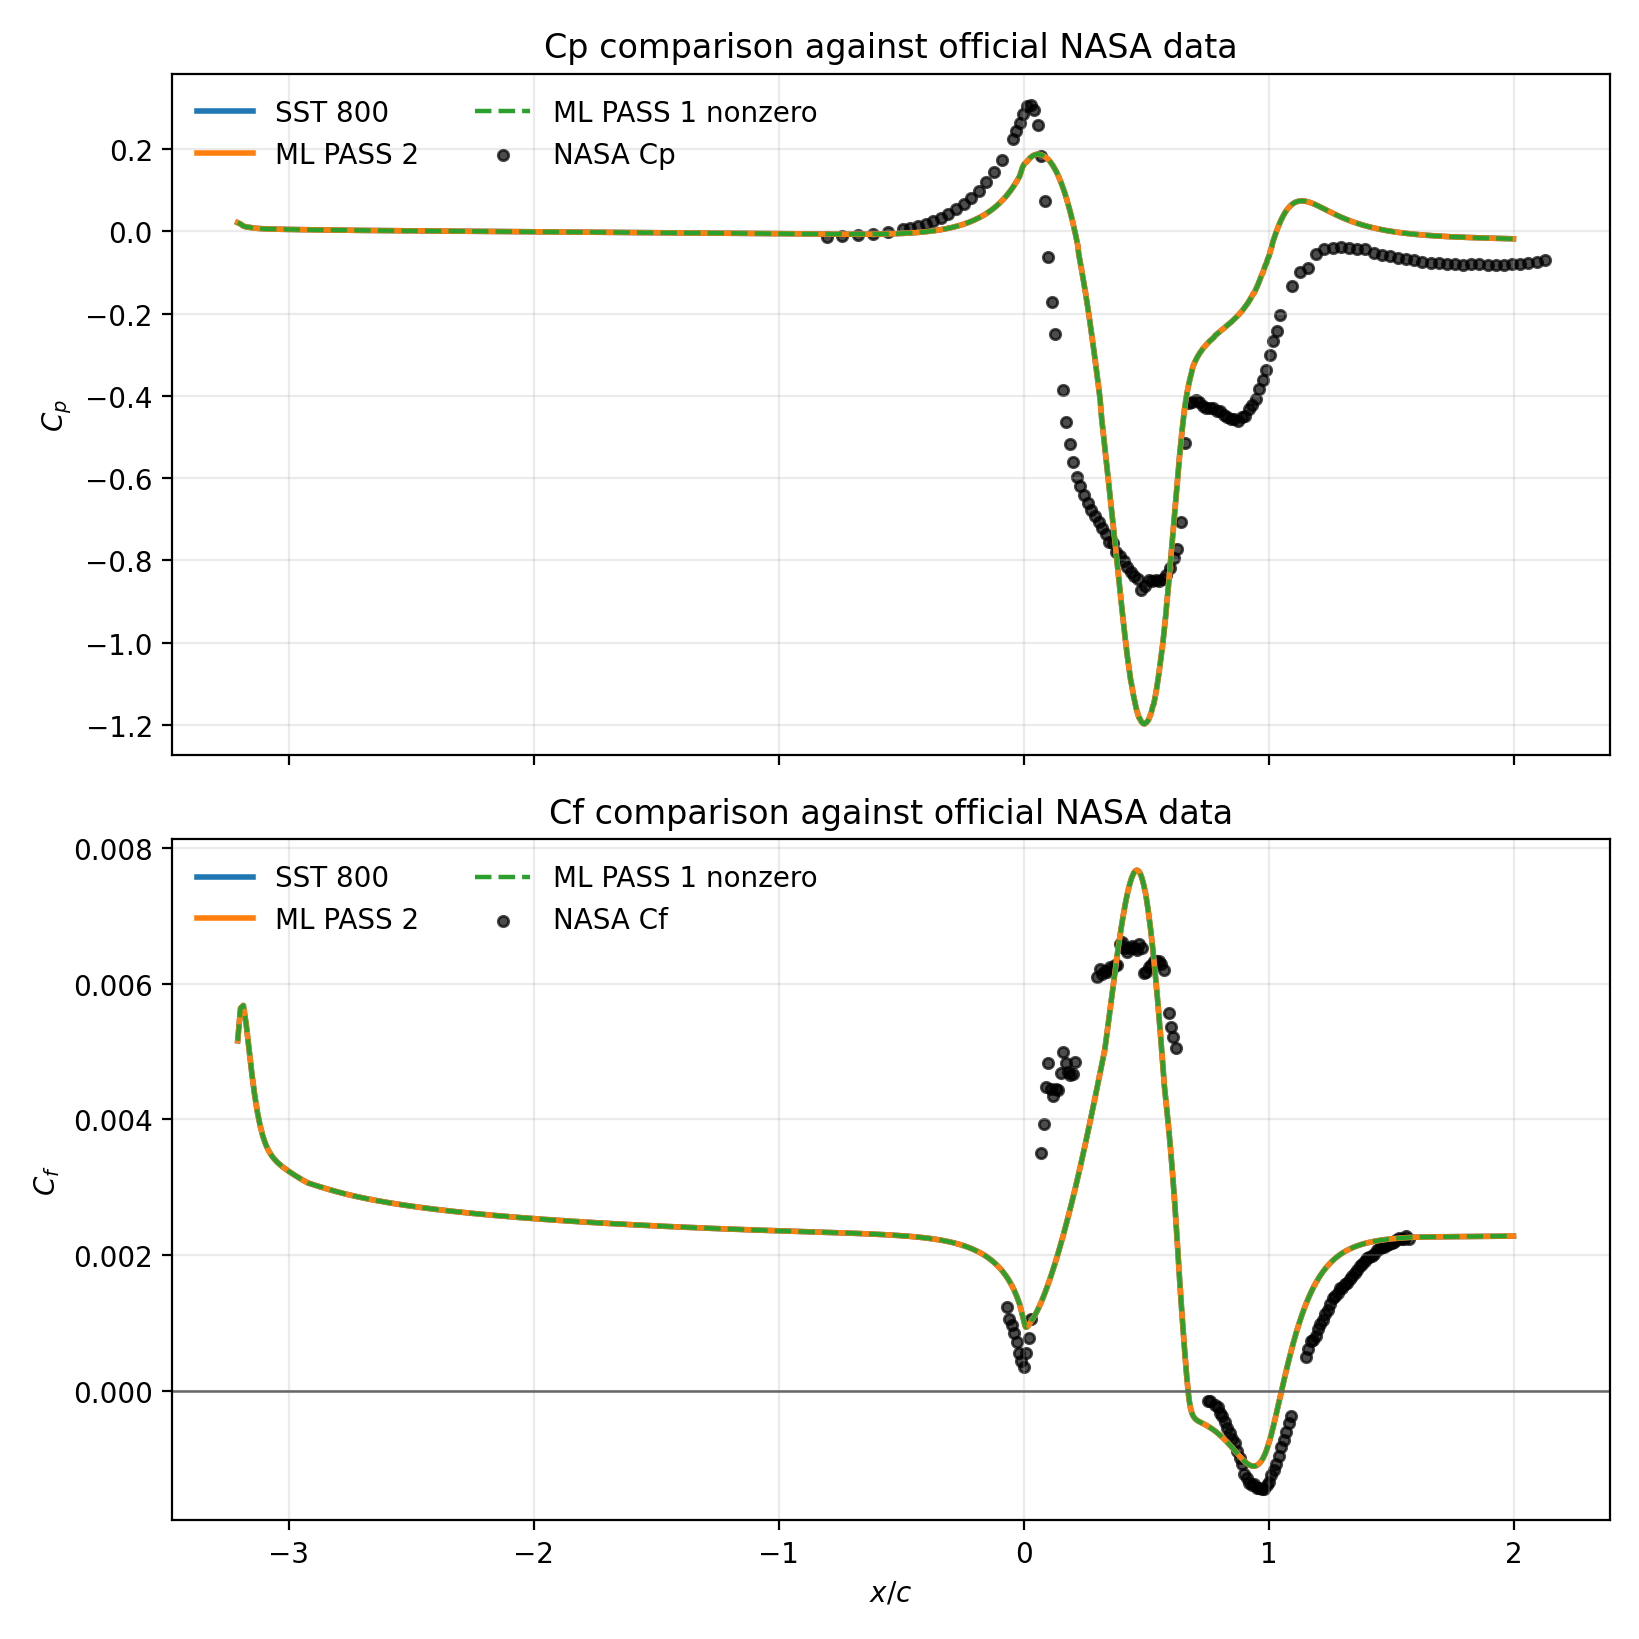
\includegraphics[width=0.94\linewidth]{figures_mlpass2/cp_cf_mlpass2.png}
\caption{Official NASA Cp and Cf comparisons for plain SST 800, ML PASS 1 nonzero, and ML PASS 2. The ML PASS 2 curves lie on top of the plain SST 800 curves to plotting precision.}
\end{figure}

\begin{figure}[H]
\centering
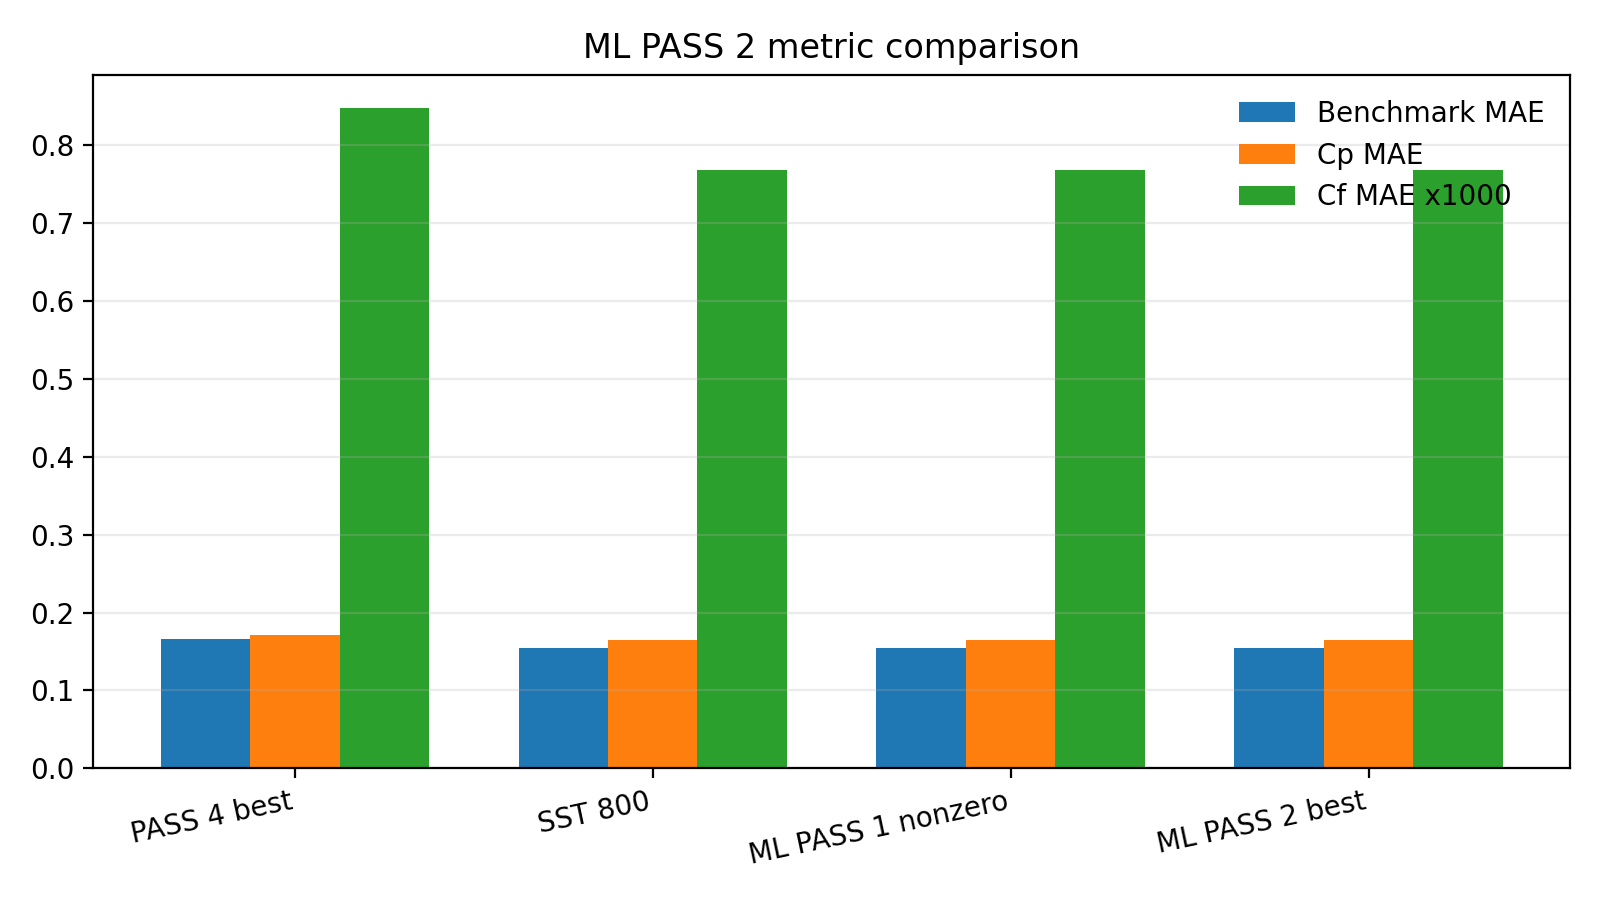
\includegraphics[width=0.90\linewidth]{figures_mlpass2/mlpass2_metric_comparison.png}
\caption{Metric comparison across the PASS 4 reference, the stronger plain SST 800 continuation, ML PASS 1, and ML PASS 2.}
\end{figure}

\begin{figure}[H]
\centering
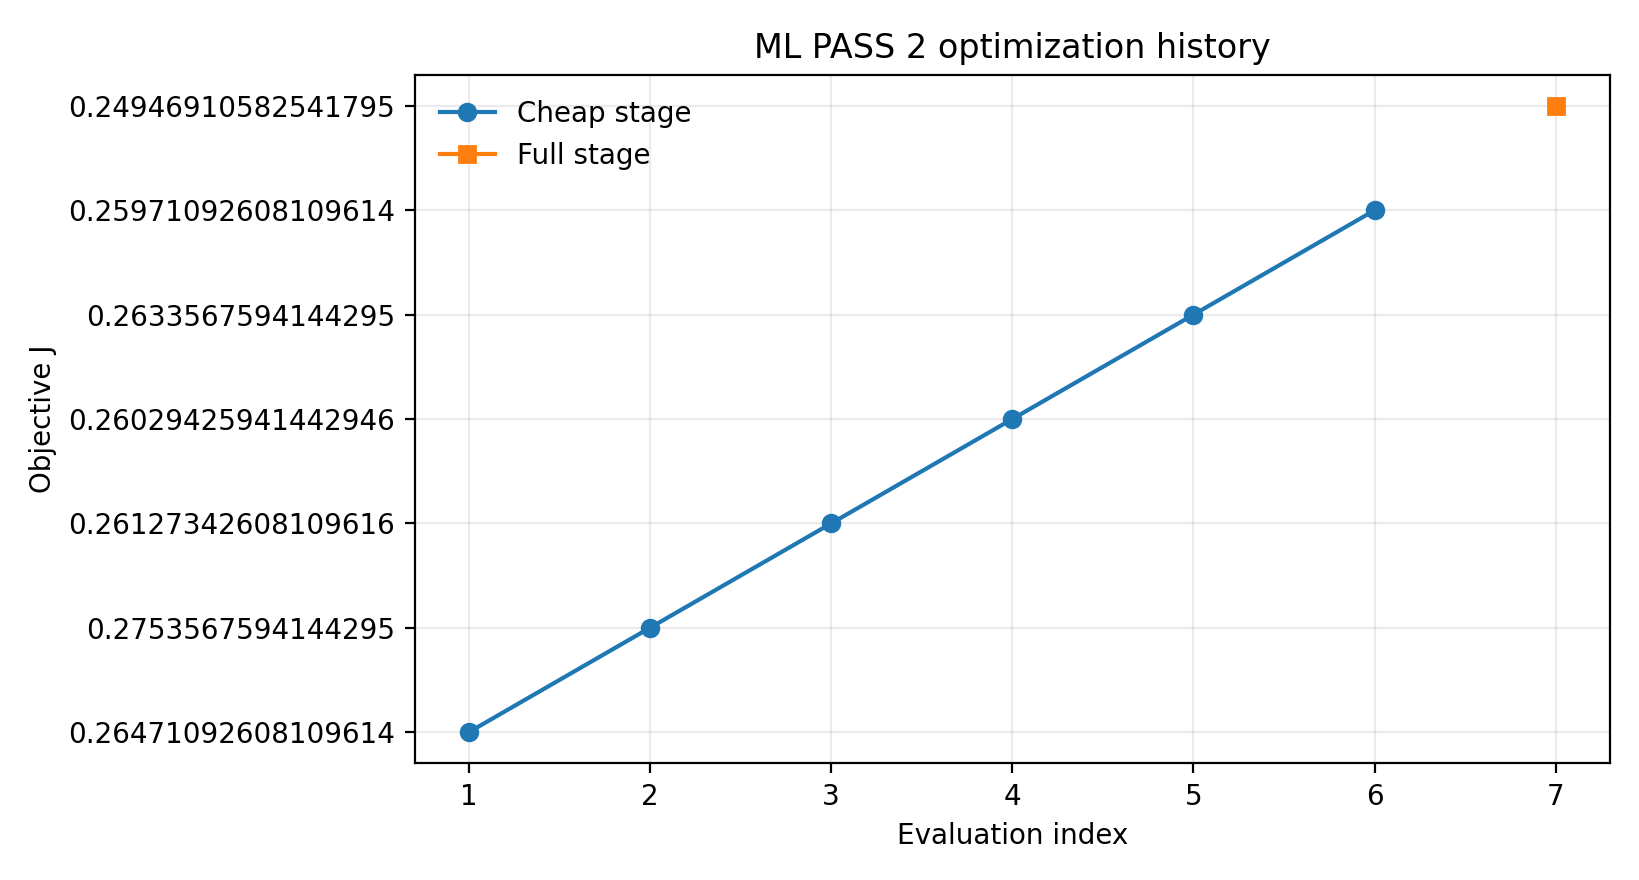
\includegraphics[width=0.90\linewidth]{figures_mlpass2/mlpass2_optimization_history.png}
\caption{ML PASS 2 optimization history. The objective changed only through regularization because the CFD metrics remained unchanged across the completed primary search.}
\end{figure}

\section{Discussion}
ML PASS 2 is a scientifically cleaner negative result than ML PASS 1. The new
method moved the correction to a more meaningful part of the closure, namely the
SST production pathway, and activated it using a separation-aware signal rather
than a generic eddy-viscosity ratio. However, on the current hump baseline that
signal was still too selective to materially change the solved flow field.

That means ML PASS 2 is \emph{more physically meaningful} than ML PASS 1, but it
is \emph{not better as a promoted model}. It does not beat the plain SST 800
continuation, and it does not improve Cp or Cf agreement.

\section{Conclusion And Recommendation}
ML PASS 2 should \textbf{not} be promoted.

The strongest reproducible conclusion is:
\begin{itemize}[leftmargin=1.2em]
\item PASS 4 / plain SST continuation remains the best ML-track benchmark
comparison baseline
\item moving the correction from a late \(\nu_t\) multiplier to the SST
production pathway was scientifically justified
\item the current separation sensor is still too weak or too selective to change
the hump solution in a useful way
\end{itemize}

The next best path, if another ML pass is attempted, is to keep the
production-side intervention but either:
\begin{itemize}[leftmargin=1.2em]
\item anchor it to a more faithful geometry / top-wall baseline first, or
\item use a broader adverse-pressure-gradient sensor with an auditable restart
workflow and lower storage overhead from the beginning
\end{itemize}

\section*{Reproducibility}
\begin{Verbatim}[fontsize=\small]
bash scripts/build_ml_hump_model.sh
bash scripts/run_nasa_hump_mlpass2.sh
MPLCONFIGDIR=docs/.mplconfig python3 scripts/make_nasa_hump_mlpass2_figures.py
bash scripts/build_report.sh
\end{Verbatim}

\end{document}
